\section{APPENDIX CHAPTER 4}\label{APPENDIX CHAPTER 4}


\subsection{Ellipse Perimeter using Ramanujan Approximation}
\label{app-chap4-Ellipse Perimeter using Ramanujan Approximation}

\noindent
Ramanujan is a well known mathematician. We used Ramanujan approximation formula to calculate the perimeter of an Ellipse. The reference is the website at URL [\href{https://www.mathsisfun.com/geometry/ellipse-perimeter.html}{Perimeter of an Ellipse}]\\

\noindent
The perimeter calculation equation for the Ellipse is given by Ramanujan as follows: 
\noindent
$Perimeter = PI*(a + b)*(1 + C/D) $ where a and b are the semi-major and semi-minor lengths, respectively. C and D are based on another variable h, defined as follows.\\

\singlespacing
\noindent
Introduce $h = (a - b)^{2} / (a + b)^{2}$ we get \\
$C = 3*h $ and $D = 10 + sqrt(4 - 3*h) $ \\

\singlespacing
\noindent
For a specific Ellipse with a = 51 and b = 11, we get\\
$h = (a - b)^{2} / (a + b)^{2}$ \\
$h = (40)^{2}/(62)^{2} = (1600)/(3844) $ \\
$h = 0.416233090530697 $\\

\singlespacing
\noindent
With h, the bvalue for C is:\\
$C = 3*h = 3*(0.416233090530697) $\\
$C = 1.24869927159209 $\\

\singlespacing
\noindent
and the value for D isd: \\
$D = 10 + sqrt(4 - 3*h) $ \\
$D = 10 + sqrt(4 - 1.24869927159209) $ \\
$D = 10 + sqrt(2.75130072840791) $\\
$D = 10 + 1.65870453318483 $ \\
$D = 11.65870453318483 $ \\

\clearpage 
\pagebreak 

\noindent
The formula for Ramanujan approximation of the perimeter on an Ellipse:\\
\noindent
$Perimeter = PI*(a + b)*(1 + C/D) $ \\

\singlespacing
\noindent
$ (C/D) = (1.24869927159209 / 11.65870453318483) $ \\
$ (C/D) = 0.107104461566707 $ \\

\singlespacing
\noindent
$Perimeter = PI*(a + b)*(1 + C/D)$ \\
$Perimeter = PI*(62)*(1 + 0.107104461566707)$ \\
$Perimeter = PI*(62)*(1.107104461566707)$ \\

\singlespacing
\noindent
Using PI = 3.141592653589793238\\
$Perimeter = 215.640417079296 $ \\
$Perimeter = 2.156404170793E+02 $ as calculated using the Ramanujan approximation formula. \\

\doublespacing
\noindent
$Perimeter = 2.156436635306E+02 $ as calculated by the parametric curve interpolation algorithm in this work for comparison. \\

%% =================================================
\clearpage
\pagebreak
%% \begin{landscape}   

\subsection{Calculation of machine epsilon C code}
\label{app4-Calculation of machine epsilon C code}

\lstset{backgroundcolor=\color{white}, basicstyle=\linespread{1.00}\footnotesize, frame={topline, bottomline, leftline, rightline}}	
\begin{lstlisting}[caption={Calculation of machine epsilon C code}, label=lst-Calculation of machine epsilon C code]	

// Calculation of machine epsilon
# include <stdio.h>
int main(void) {
	
  float         floatMachep   = 1.0;
  double        doubleMachep  = 1.0;
  long double   longDblMachep = 1.0;
	
  while (1.0 + floatMachep/2.0 != 1.0) {
	floatMachep /= 2.0;
  }
  while (1.0 + doubleMachep/2.0 != 1.0) {
	doubleMachep /= 2.0;
  }
  while (1.0 + longDblMachep/2.0 != 1.0) {
	longDblMachep /= 2.0;
  }

  printf("Machine Epsilon float type\t= %.19e\n", floatMachep);
  printf("Machine Epsilon double type\t= %.19e\n", doubleMachep);
  printf("Machine Epsilon long double type\t= %.19Le\n", longDblMachep);
	
  return(0);
}
/*
COMPILATION  
wruslan@HP-Laptop-01:~$ gcc -o calculate-machep.cx calculate-machep.c 

EXECUTION
wruslan@HP-Laptop-01:~$ ./calculate-machep.cx 
Machine Epsilon float type       = 2.2204460492503130808e-16 
Machine Epsilon double type      = 2.2204460492503130808e-16 
Machine Epsilon long double type = 1.0842021724855044340e-19 
wruslan@HP-Laptop-01:~$ 
*/
\end{lstlisting}
%% \end{landscape}   

%% =================================================
\clearpage
\pagebreak

\subsection{Ranges of floating-point numbers in C code}
\label{app4-Ranges of floating-point numbers in C code}

\lstset{backgroundcolor=\color{white}, basicstyle=\linespread{1.00}\footnotesize, frame={topline, bottomline, leftline, rightline}}	
\begin{lstlisting}[caption={Display ranges of floating-point and integer numbers}, label=lst-Display ranges of floating-point and integer numbers]	
// Display ranges of floating-point and integer numbers
# include <stdio.h>
# include <limits.h> 
# include <float.h>
int main(void) {
	
	printf("Minimum float  \t\t= %.12e \n", FLT_MIN);
	printf("Maximum float  \t\t= %.12e \n", FLT_MAX);
	
	printf("Minimum double \t\t= %.12e \n", DBL_MIN);
	printf("Maximum double \t\t= %.12e \n", DBL_MAX);
	
	printf("Minimum long double \t= %.12Le \n", LDBL_MIN);
	printf("Maximum long double \t= %.12Le \n", LDBL_MAX);
	
	printf("Minimum short       \t= %d \n", SHRT_MIN);
	printf("Maximun short       \t= %d \n", SHRT_MAX);
	printf("Maximum ushort      \t= %ud \n", USHRT_MAX);
	
	printf("Minimum int         \t= %d \n", INT_MIN);
	printf("Maximum int         \t= %d \n", INT_MAX);
	printf("Maximum uint        \t= %ud \n", UINT_MAX);
	
	printf("Minimum long int    \t= %li \n", LONG_MIN);
	printf("Maximum long int    \t= %li \n", LONG_MAX);
	printf("Maximum ulong int   \t= %lu \n", ULONG_MAX);
	
	return(0);
}
/*
COMPILATION
wruslan@HP-Laptop-01:~$ 
     gcc -o ranges-numbers-c-code.cx ranges-numbers-c-code.c 
EXECUTION
wruslan@HP-Laptop-01:~$ ./ranges-numbers-c-code.cx 
Minimum float           = 1.175494350822e-38 
Maximum float           = 3.402823466385e+38 
Minimum double          = 2.225073858507e-308 
Maximum double          = 1.797693134862e+308 
Minimum long double 	= 3.362103143112e-4932 
Maximum long double 	= 1.189731495357e+4932 
Minimum short       	= -32768 
Maximun short       	= 32767 
Maximum ushort      	= 65535d 
Minimum int         	= -2147483648 
Maximum int         	= 2147483647 
Maximum uint        	= 4294967295d 
Minimum long int    	= -9223372036854775808 
Maximum long int    	= 9223372036854775807 
Maximum ulong int   	= 18446744073709551615 
wruslan@HP-Laptop-01:~$ 
*/
\end{lstlisting}


%% =================================================
\clearpage
\pagebreak

\subsection{Machine epsilon affecting addition and subtraction operations}
\label{app4-Machine epsilon affecting addition and subtraction operations}

\lstset{backgroundcolor=\color{white}, basicstyle=\linespread{1.00}\footnotesize, frame={topline, bottomline, leftline, rightline}}	
\begin{lstlisting}[caption={Machine epsilon affecting addition and subtraction operations}, label=lst-Machine epsilon affecting addition and subtraction operations]	
// Machine epsilon affecting addition and subtraction operations
# include <stdio.h>
# include <limits.h> 
# include <float.h>
int main(void) {
 double largeDouble  = 3.123456789E+6;
 double smallDouble  = 1.123456789E-18;      // BELOW MACHINE  EPSILON 
 printf("\n(1) ADDITION OF SMALL NUMBER BELOW MACHINE EPSILON \n");
 printf("  largeDouble %.12e \n", largeDouble); 
 printf("+ smallDouble %.12e \n", smallDouble);
 printf("=             %.12e \n", (largeDouble + smallDouble));
 printf("\n(2) SUBTRACTION OF SMALL NUMBER BELOW MACHINE EPSILON \n");
 printf("  largeDouble %.12e \n", largeDouble); 
 printf("- smallDouble %.12e \n", smallDouble);
 printf("=             %.12e \n", (largeDouble - smallDouble));
 printf("\n(3) MULTIPLICATION BY SMALL NUMBER BELOW MACHINE EPSILON\n");
 printf("  largeDouble %.12e \n", largeDouble); 
 printf("* smallDouble %.12e \n", smallDouble);
 printf("=             %.12e \n", (largeDouble * smallDouble));
 printf("\n(4) DIVISION BY SMALL NUMBER BELOW MACHINE EPSILON \n");
 printf("  largeDouble %.12e \n", largeDouble); 
 printf("/ smallDouble %.12e \n", smallDouble);
 printf("=             %.12e \n", (largeDouble / smallDouble));
 return(0);
}
/*
COMPILATION
wruslan@HP-Laptop-01:~$ 
gcc -o fixing-machine-epsilon.cx fixing-machine-epsilon.c 
EXECUTION
wruslan@HP-Laptop-01:~$ ./fixing-machine-epsilon.cx 

(1) ADDITION OF SMALL NUMBER BELOW MACHINE EPSILON 
  largeDouble 3.123456789000e+06 
+ smallDouble 1.123456789000e-18 
=             3.123456789000e+06 

(2) SUBTRACTION OF SMALL NUMBER BELOW MACHINE EPSILON 
  largeDouble 3.123456789000e+06 
- smallDouble 1.123456789000e-18 
=             3.123456789000e+06 

(3) MULTIPLICATION BY SMALL NUMBER BELOW MACHINE EPSILON 
  largeDouble 3.123456789000e+06 
* smallDouble 1.123456789000e-18 
=             3.509068734750e-12 

(4) DIVISION BY SMALL NUMBER BELOW MACHINE EPSILON 
  largeDouble 3.123456789000e+06 
/ smallDouble 1.123456789000e-18 
=             2.780219782000e+24 
*/
wruslan@HP-Laptop-01:~$ 
\end{lstlisting}

%% =================================================
\clearpage
\pagebreak

\subsection{Resolving machine epsilon issue}
\label{app4-Resolving machine epsilon issue}

\lstset{backgroundcolor=\color{white}, basicstyle=\linespread{1.00}\footnotesize, frame={topline, bottomline, leftline, rightline}}	
\begin{lstlisting}[caption={Resolving machine epsilon issue}, label=lst-Resolving machine epsilon issue]	
# include <stdio.h>
# include <limits.h> 
# include <float.h>
int main(void) {
	
 double largeDouble  = 3.123456789E+6;
 double smallDouble  = 1.123456789E-18;    // BELOW MACHINE EPSILON 
 double machepFactor = 1.8765E+10;         // A LARGE POSITIVE NUMBER
	
 printf("ADDITION OF SMALL NUMBER BELOW MACHINE EPSILON \n");
 printf("  largeDouble   %.12e \n", largeDouble); 
 printf("+ smallDouble   %.12e \n", smallDouble);
 printf("=               %.12e \n", (largeDouble + smallDouble));
	
 double uplargeDouble = (machepFactor)*largeDouble;
 double upsmallDouble = (machepFactor)*smallDouble;
	
 printf("\n");
 printf("uplargeDouble   %.12e \n", uplargeDouble);    
 printf("upsmallDouble   %.12e \n", upsmallDouble);    
	
 double the_SUM_01 = (uplargeDouble + upsmallDouble);
 double the_SUM_02 = (the_SUM_01)/(machepFactor);
	
 printf("the_SUM_01 =    %.12e \n", the_SUM_01);      
 printf("the_SUM_02 =    %.12e \n", the_SUM_02); 
	
 return(0);
}
/*
COMPILATION
wruslan@HP-Laptop-01:~$ 
gcc -o Resolving-machine-epsilon.cx Resolving-machine-epsilon.c 

EXECUTION
wruslan@HP-Laptop-01:~$ ./Resolving-machine-epsilon.cx 

ADDITION OF SMALL NUMBER BELOW MACHINE EPSILON 
  largeDouble   3.123456789000e+06 
+ smallDouble   1.123456789000e-18 
=               3.123456789000e+06 

uplargeDouble   5.861166664558e+16 
upsmallDouble   2.108166664558e-08 
the_SUM_01 =    5.861166664558e+16 
the_SUM_02 =    3.123456789000e+06 

wruslan@HP-Laptop-01:~$ 
*/
\end{lstlisting}




%% =================================================
\clearpage
\pagebreak

\subsection{LinuxCNC Validation of Curves}\label{LinuxCNC Validation of Curves}

The following list provides the links to the screen capture of real runs of the G-codes generated by the interpolation algorithm on the LinuxCNC-Axis control computer. The computer drives a CNC machine by sending electrical signals via the standard parallel port. The figures in the next ten(10) pages are provided in landscape mode.


\begin{enumerate}
	\item Circle curve validation link [\ref{img-Circle validation LinuxCNC-Axis execution}]
	\item Ellipse curve validation link  [\ref{img-Ellipse validation LinuxCNC-Axis execution}]
	\item Teardrop curve validation link  [\ref{img-Teardrop validation LinuxCNC-Axis execution}]
	\item Butterfly curve validation link  [\ref{img-Butterfly validation LinuxCNC-Axis execution}]
	\item Snailshell curve validation link [\ref{img-Snailshell validation LinuxCNC-Axis execution}]
	\item Skewed-Astroid curve validation link  [\ref{img-Skewed-Astroid validation LinuxCNC-Axis execution}]
	\item Ribbon-10L curve validation link  [\ref{img-Ribbon-10L validation LinuxCNC-Axis execution}]
	\item Ribbon-100L curve validation link  [\ref{img-Ribbon-100L validation LinuxCNC-Axis execution}]
	\item AstEpi curve validation link [\ref{img-AstEpi validation LinuxCNC-Axis execution}]
	\item SnaHyp curve validation link [\ref{img-SnaHyp validation LinuxCNC-Axis execution}]
\end{enumerate}


%% ===================================================================
%% 1 CIRCLE LINUXCNC SIMULATION IMAGE
%% ==================================
\clearpage
\pagebreak
\begin{landscape}
	
	\begin{figure}
		\centering
		\caption  {Circle validation LinuxCNC-Axis execution}
		\label{img-Circle validation LinuxCNC-Axis execution}
		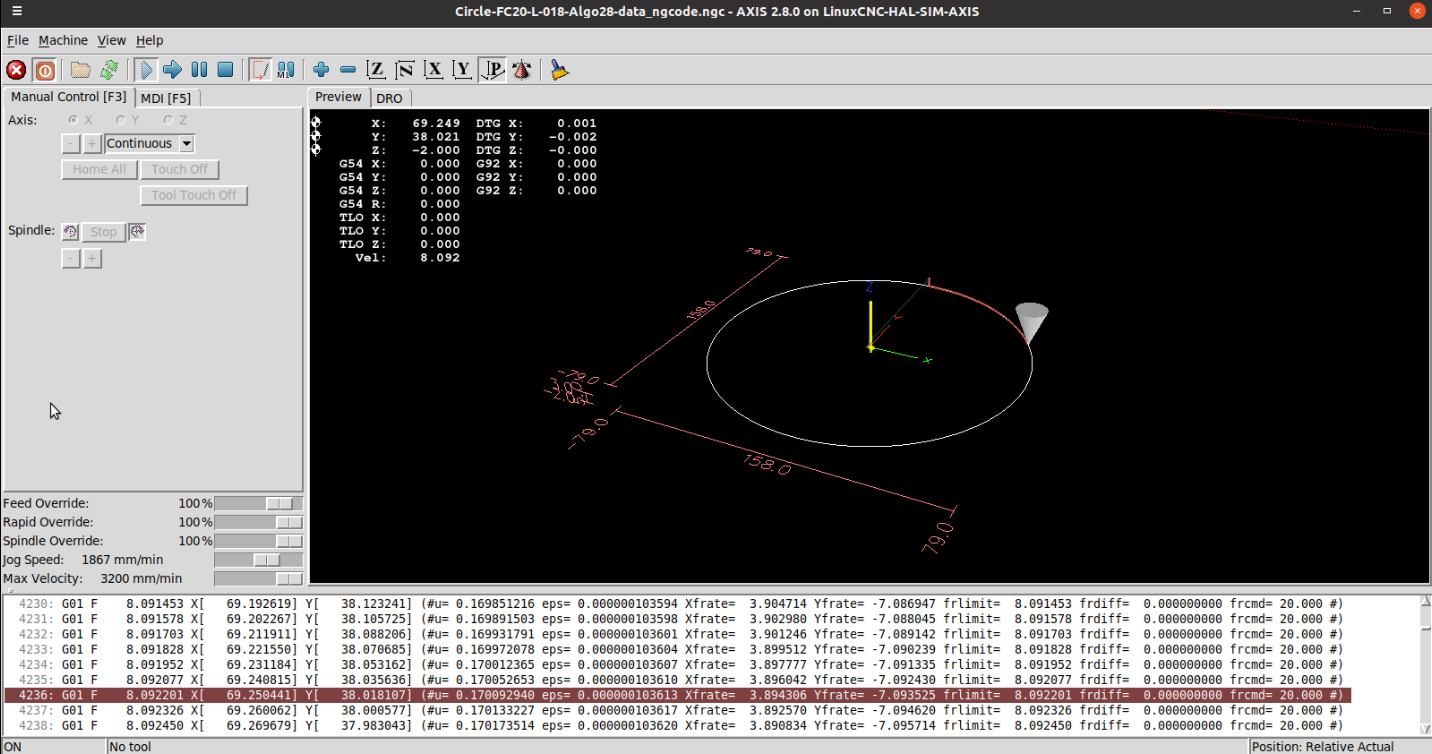
\includegraphics[width=1.65\textwidth]{Chap4/Validation/Circle/Circle-FC20-L-018-Algo28-CNC-Validation-Screenshot_2023-10-09_09-46-06.png} 
	\end{figure}
	
	
\end{landscape}

%% 2 ELLIPSE LINUXCNC
%% ==================================
\clearpage
\pagebreak
\begin{landscape}
	
	\begin{figure}
		\centering
		\caption  {Ellipse validation LinuxCNC-Axis execution}
		\label{img-Ellipse validation LinuxCNC-Axis execution}
		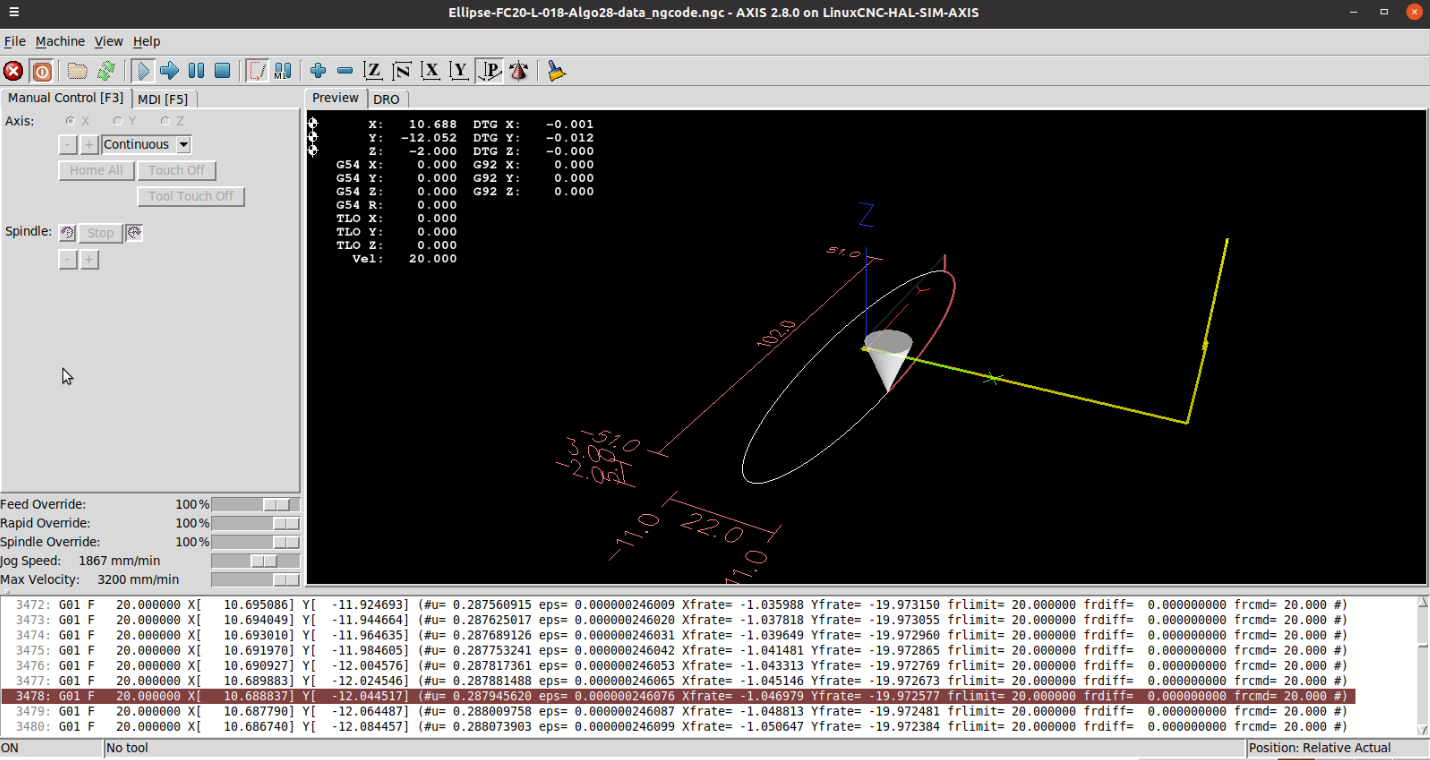
\includegraphics[width=1.65\textwidth]{Chap4/Validation/Ellipse/Ellipse-FC20-L-018-Algo28-CNC-Validation-Screenshot_2023-10-09_09-56-34.png} 
	\end{figure}
	
	
\end{landscape}

%% 3 TEARDROP LINUXCNC
%% ==================================
\clearpage
\pagebreak
\begin{landscape}
	
	\begin{figure}
		\centering
		\caption  {Teardrop validation LinuxCNC-Axis execution}
		\label{img-Teardrop validation LinuxCNC-Axis execution}
		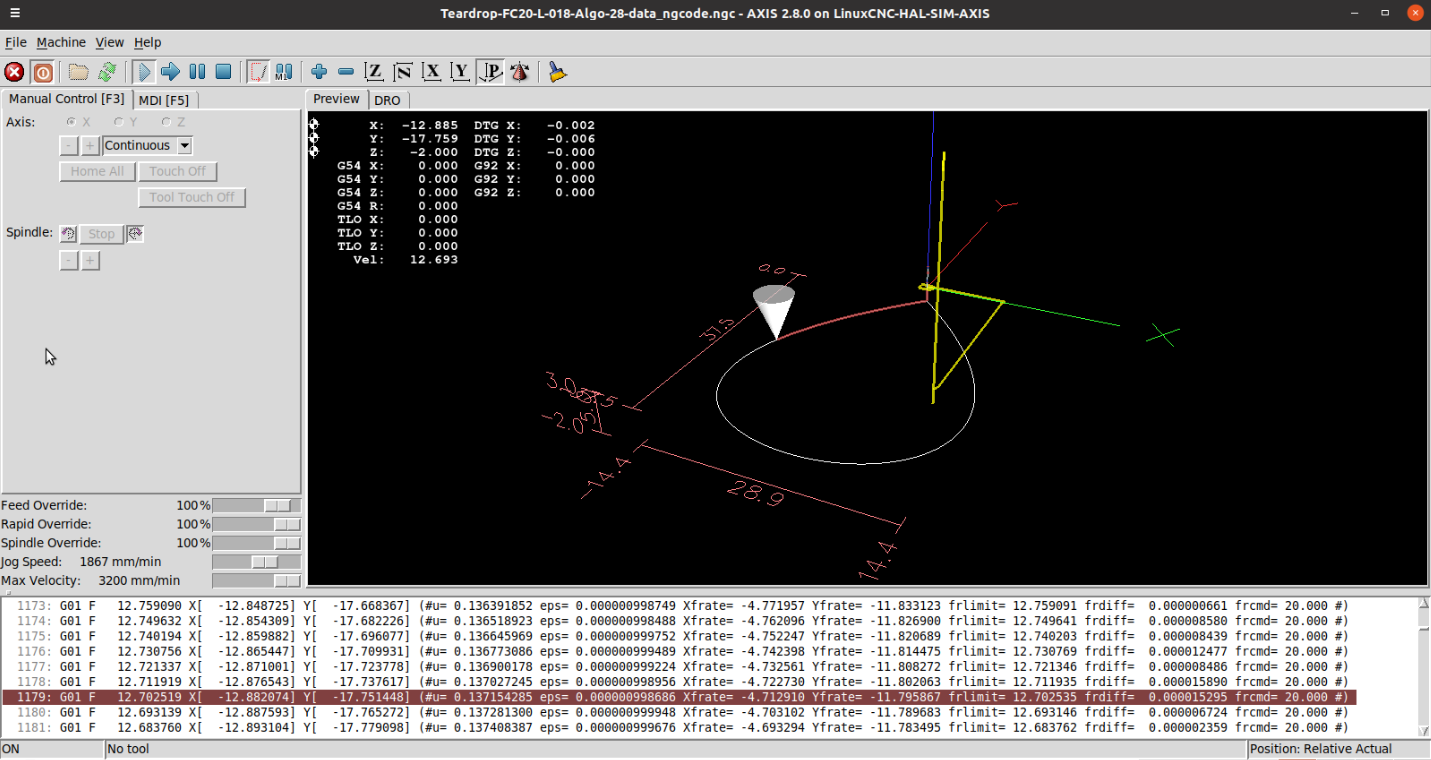
\includegraphics[width=1.65\textwidth]{Chap4/Validation/Teardrop/Teardrop-FC20-L-018-Algo28-CNC-Validation-Screenshot_2023-10-09_10-00-49.png} 
	\end{figure}
	
\end{landscape}

%% 4 BUTTERFLY LINUXCNC
%% ==================================
\clearpage
\pagebreak
\begin{landscape}
	
	\begin{figure}
		\centering
		\caption  {Butterfly validation LinuxCNC-Axis execution}
		\label{img-Butterfly validation LinuxCNC-Axis execution}
		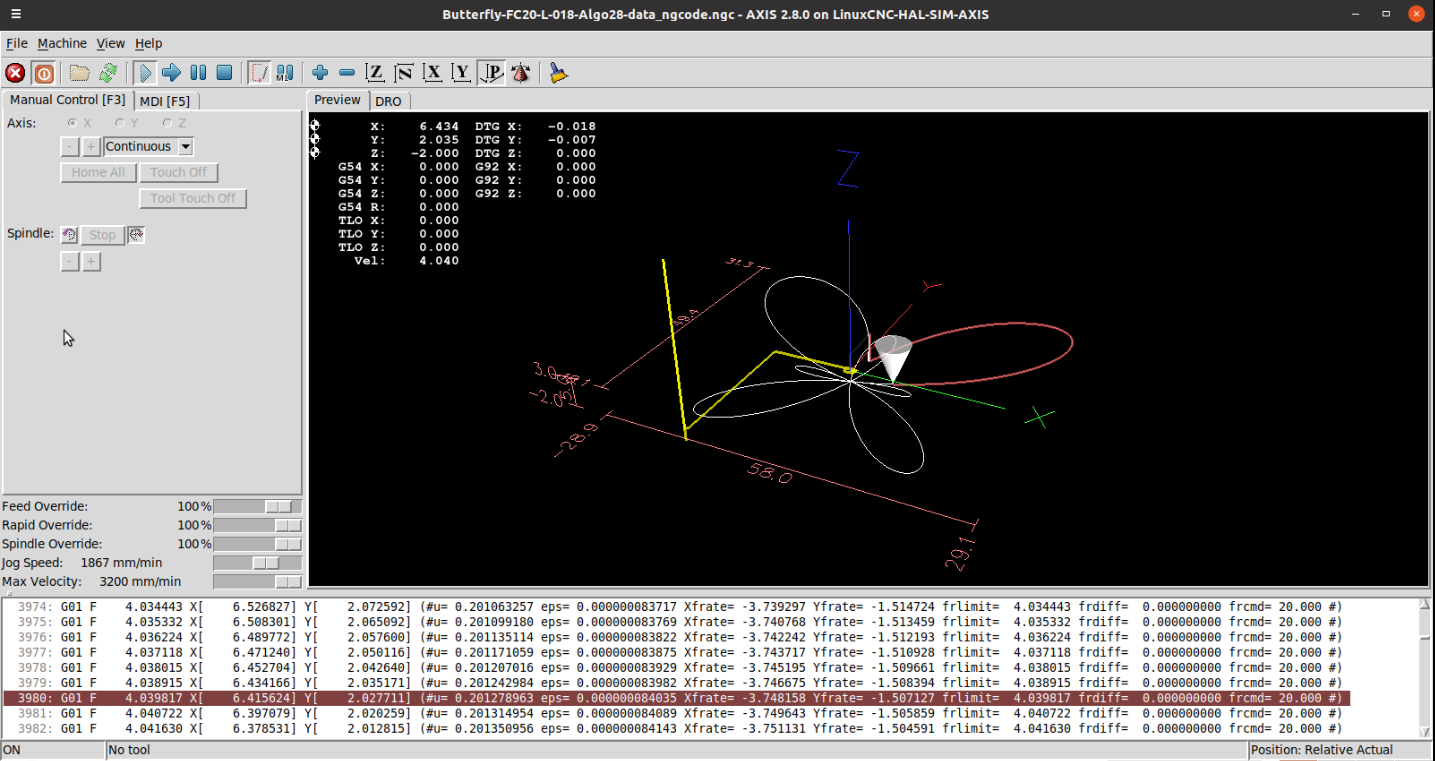
\includegraphics[width=1.65\textwidth]{Chap4/Validation/Butterfly/Butterfly-FC20-L-018-Algo28-CNC-Validation-Screenshot_2023-10-09_10-19-54.png} 
	\end{figure}	
	
\end{landscape}

%% 5 SNAILSHELL LINUXCNC
%% ==================================
\clearpage
\pagebreak
\begin{landscape}
	
	\begin{figure}
		\centering
		\caption  {Snailshell validation LinuxCNC-Axis execution}
		\label{img-Snailshell validation LinuxCNC-Axis execution}
		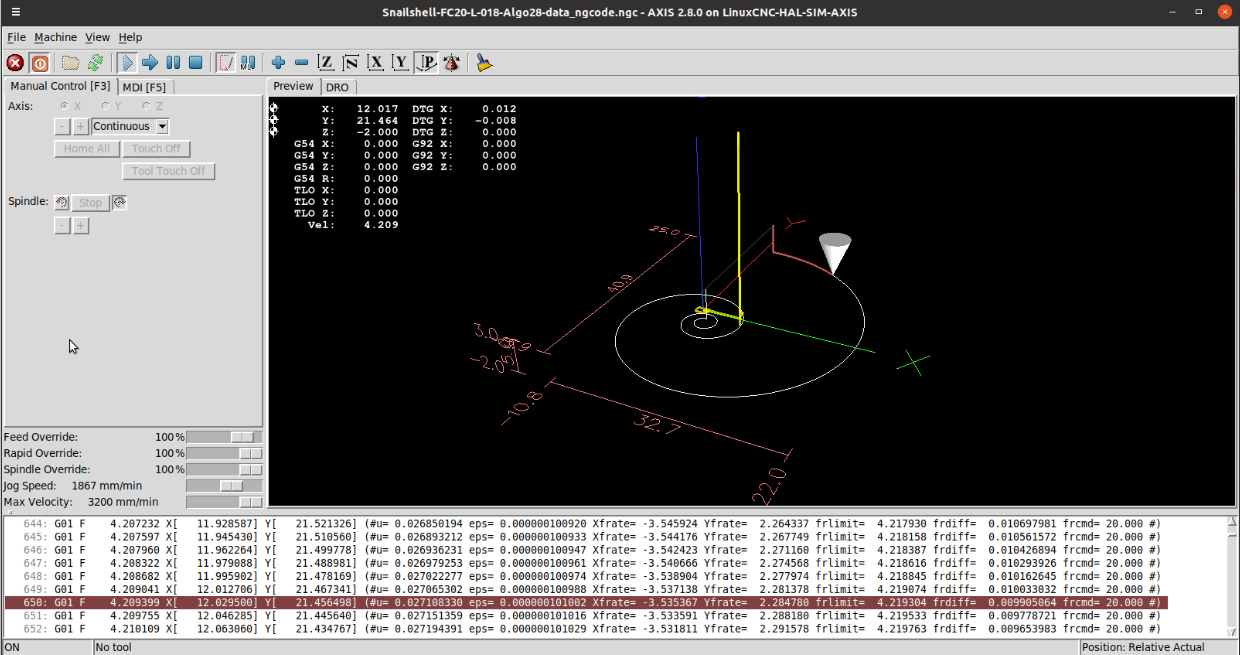
\includegraphics[width=1.65\textwidth]{Chap4/Validation/Snailshell/Snailshell-FC20-L-018-Algo28-CNC-Validation-Screenshot_2023-10-09_10-25-28.png} 
	\end{figure}	
	
\end{landscape}

%% 6 SKEWEED-ASTROID
%% ==================================
\clearpage
\pagebreak
\begin{landscape}
	
	\begin{figure}
		\centering
		\caption  {Skewed-Astroid validation LinuxCNC-Axis execution}
		\label{img-Skewed-Astroid validation LinuxCNC-Axis execution}
		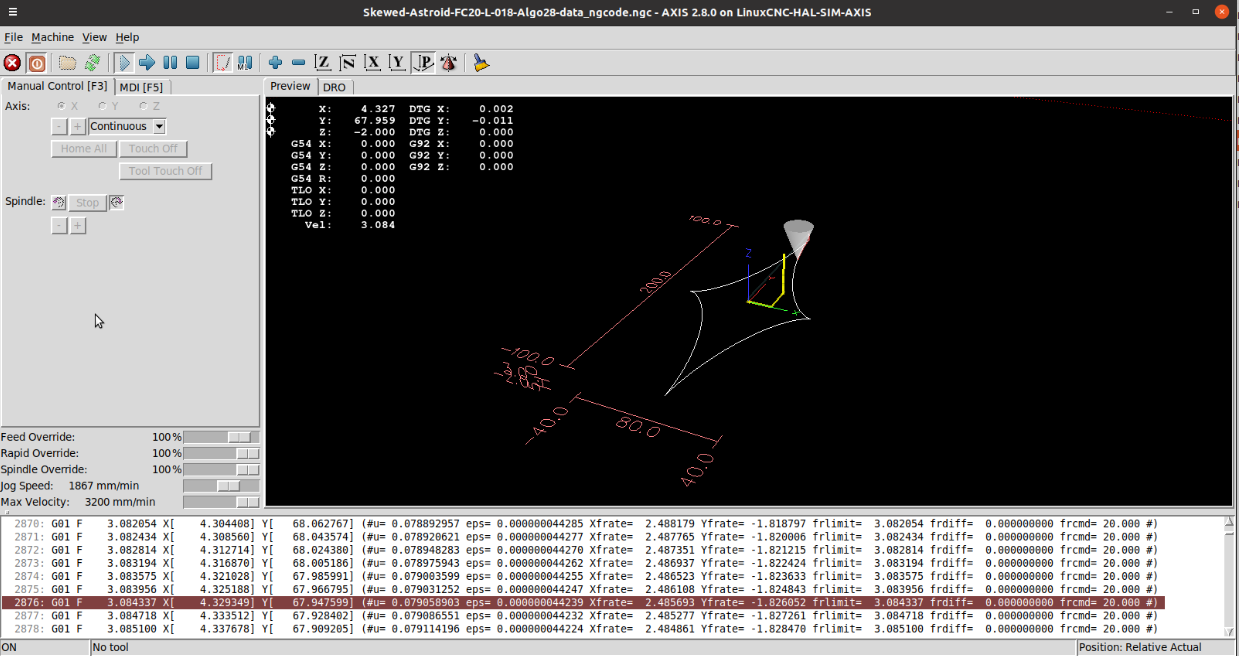
\includegraphics[width=1.65\textwidth]{Chap4/Validation/Skewed-Astroid/Skewed-Astroid-FC20-L-018-Algo28-CNC-Validation-Screenshot_2023-10-09_10-38-31.png} 
	\end{figure}	
	
\end{landscape}


%% 7 RIBBON-10L LINUXCNC
%% ==================================
\clearpage
\pagebreak
\begin{landscape}
	
	\begin{figure}
		\centering
		\caption  {Ribbon-10L validation LinuxCNC-Axis execution}
		\label{img-Ribbon-10L validation LinuxCNC-Axis execution}
		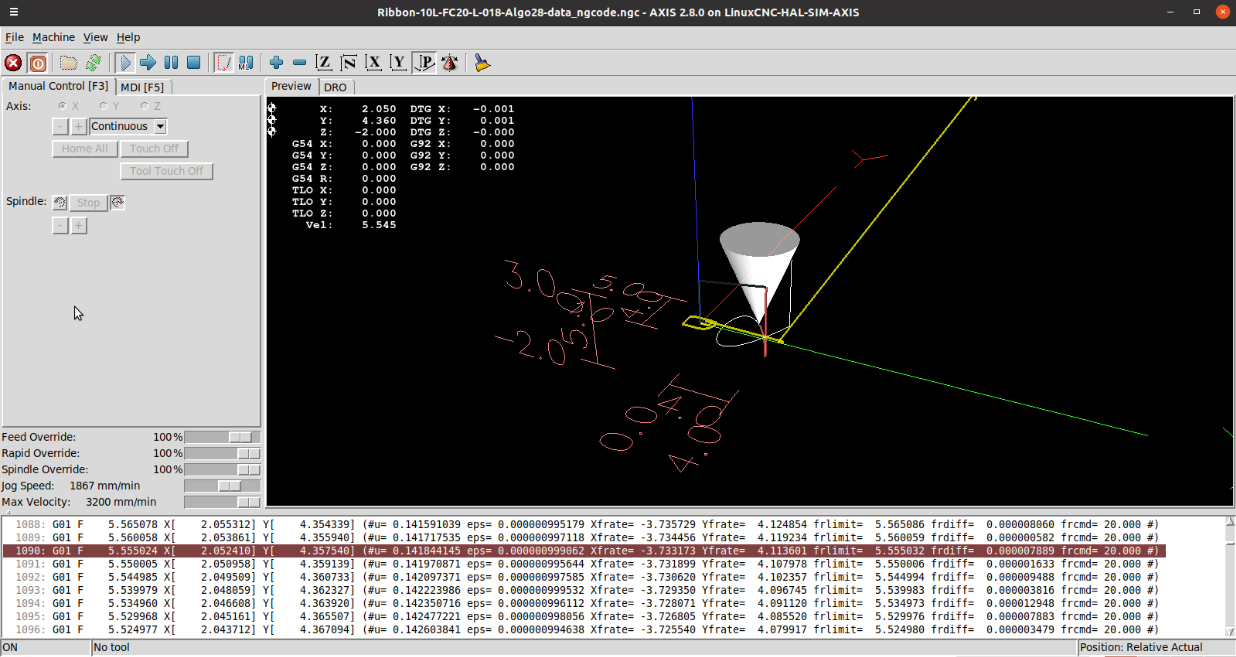
\includegraphics[width=1.65\textwidth]{Chap4/Validation/Ribbon-10L/Ribbon-10L-FC20-L-018-Algo28-CNC-Validation-Screenshot_2023-10-09_10-41-05.png} 
	\end{figure}	
	
\end{landscape}

%% 8 RIBBON-100 LINUXCNC
%% ==================================
\clearpage
\pagebreak
\begin{landscape}
	
	\begin{figure}
		\centering
		\caption  {Ribbon-100L validation LinuxCNC-Axis execution}
		\label{img-Ribbon-100L validation LinuxCNC-Axis execution}
		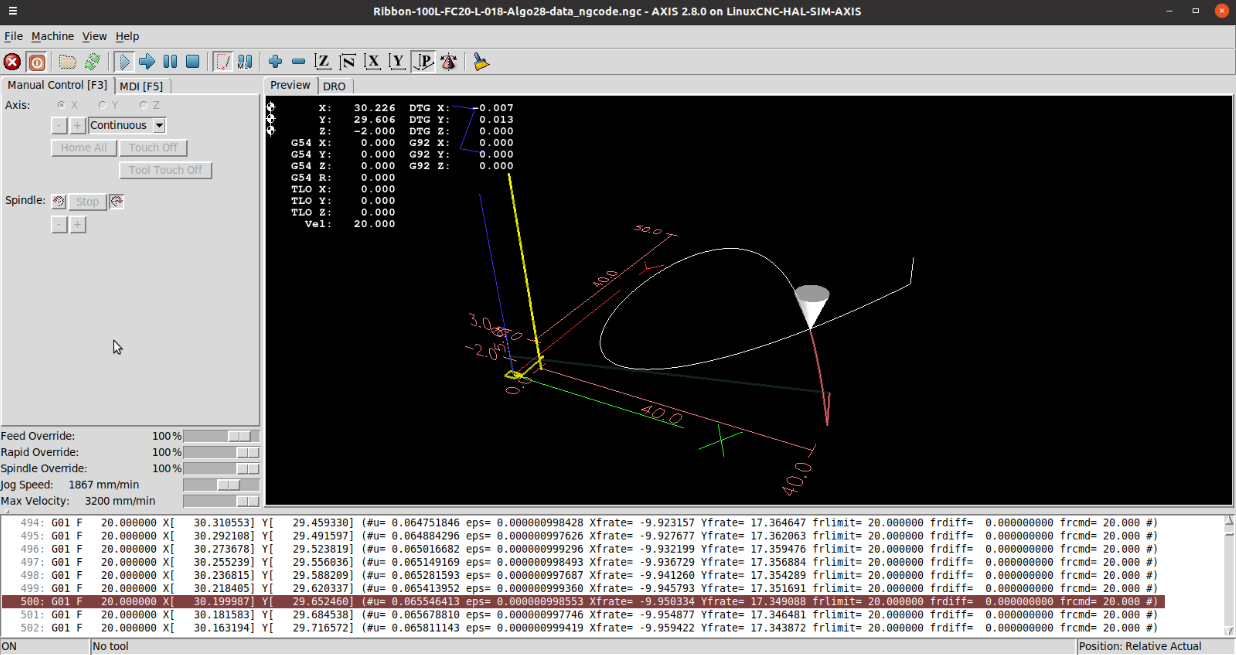
\includegraphics[width=1.65\textwidth]{Chap4/Validation/Ribbon-100L/Ribbon-100L-FC20-L-018-Algo28-CNC-Validation-Screenshot_2023-10-09_10-45-00.png} 
	\end{figure}	
	
\end{landscape}


%% 9 ASTEPI LINUXCNC
%% ==================================
\clearpage
\pagebreak
\begin{landscape}
	
	\begin{figure}
		\centering
		\caption  {AstEpi validation LinuxCNC-Axis execution}
		\label{img-AstEpi validation LinuxCNC-Axis execution} 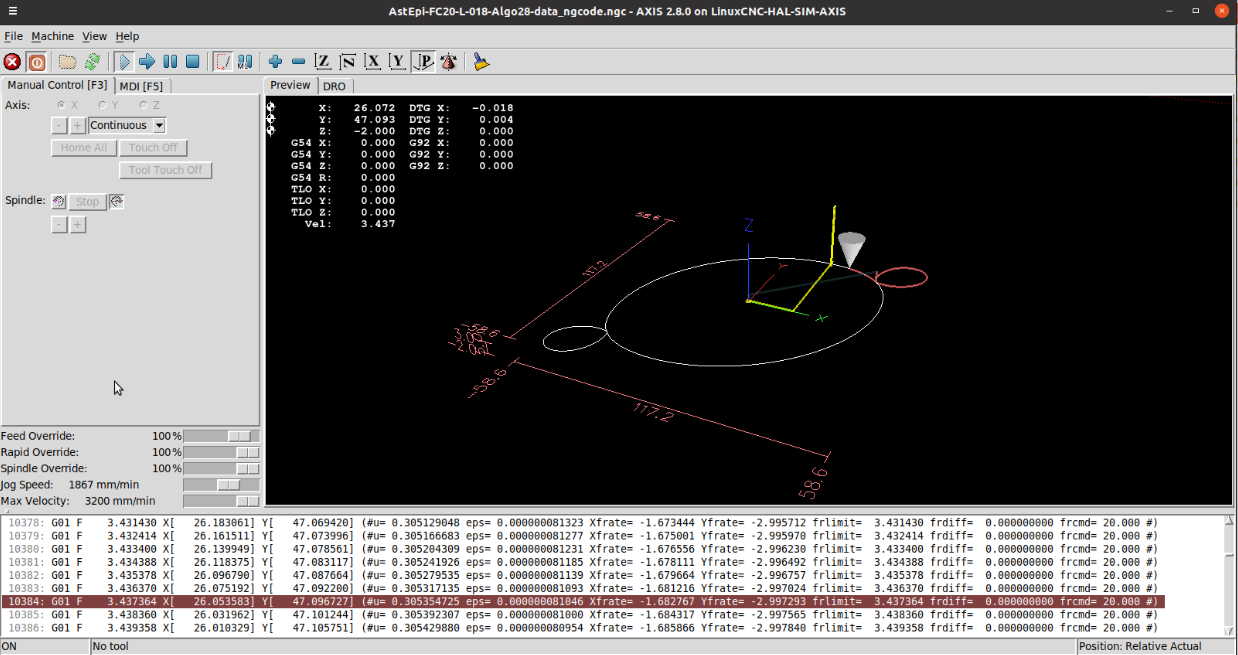
\includegraphics[width=1.65\textwidth]{Chap4/Validation/AstEpi/AstEpi-FC20-L-018-Algo28-CNC-Validation-Screenshot_2023-10-09_11-01-23.png} 
	\end{figure}
	
\end{landscape}

%% 10 SHAHYP LINUXCNC
%% ==================================
\clearpage
\pagebreak
\begin{landscape}
	
	\begin{figure}
		\centering
		\caption  {SnaHyp validation LinuxCNC-Axis execution}
		\label{img-SnaHyp validation LinuxCNC-Axis execution} 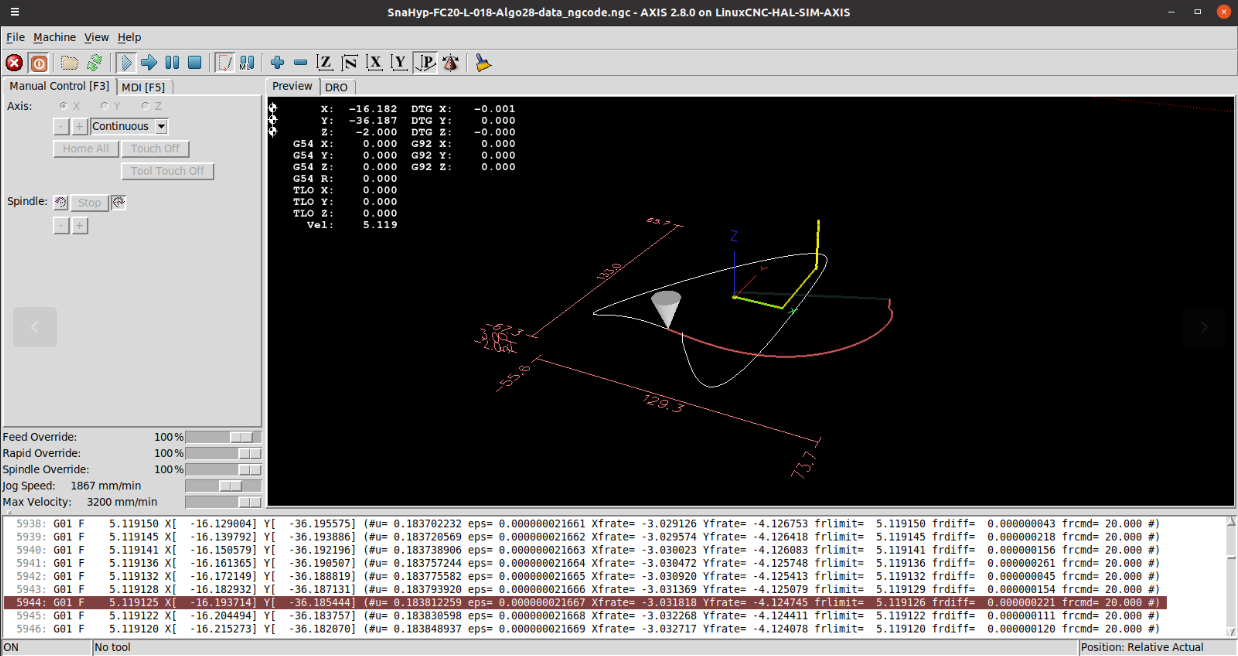
\includegraphics[width=1.65\textwidth]{Chap4/Validation/SnaHyp/SnaHyp-FC20-L-018-Algo28-CNC-Validation-Screenshot_2023-10-09_11-30-38.png} 
	\end{figure}
	
\end{landscape}

\clearpage
\pagebreak